\documentclass[12pt,a4paper]{report}
\usepackage[utf8]{inputenc}
\usepackage[T1]{fontenc}
\usepackage{graphicx}
\usepackage{tikz}
\usetikzlibrary{positioning}
\usepackage{xcolor}
\usepackage{geometry}
\usepackage{hyperref}
\usepackage{enumitem}
\usepackage{booktabs}

\geometry{margin=1in}

\title{\textbf{Section X: Cybersecurity \& Cyber-Resilience Strategy for Sovereign Cloud/Edge Computing}}
\author{}
\date{}

\begin{document}

\maketitle

\tableofcontents
\newpage

\begin{figure}[h!]
		\centering
		\resizebox{\textwidth}{!}{%
		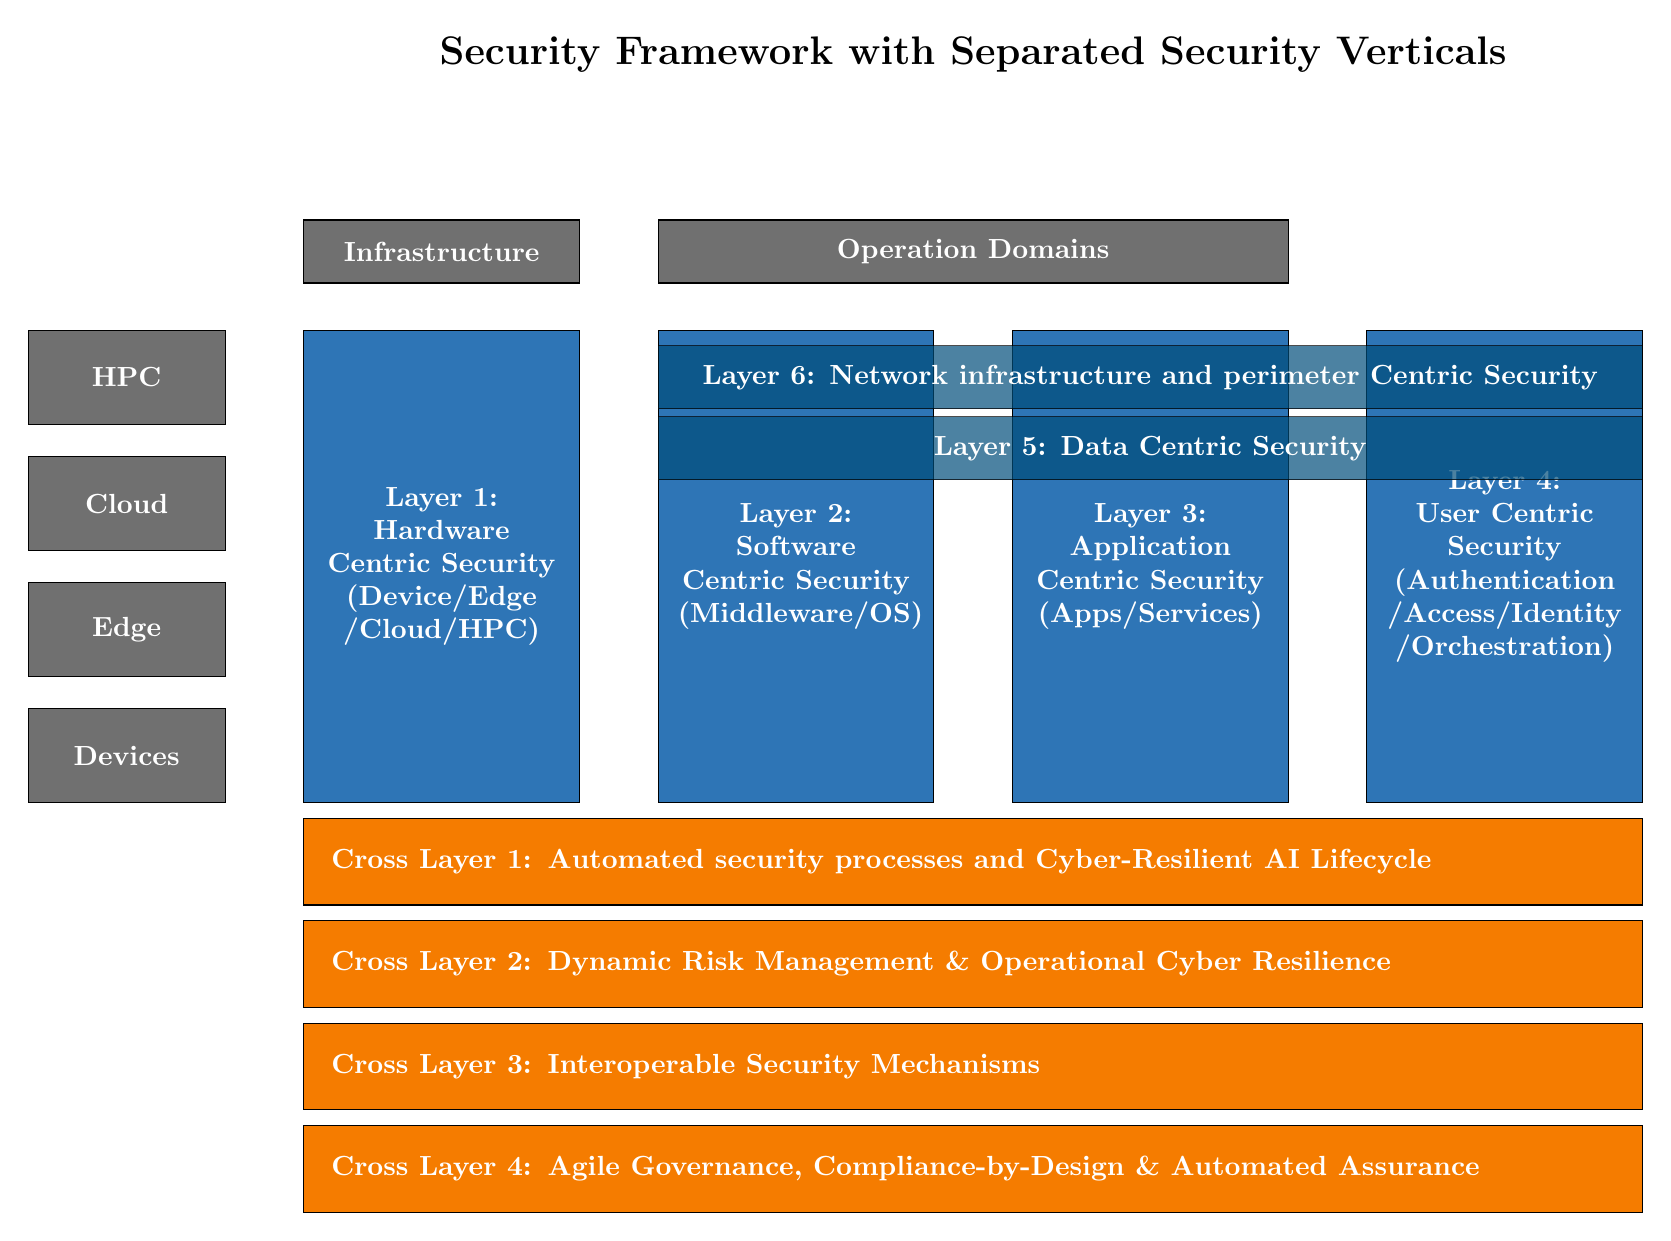
\begin{tikzpicture}[every node/.style={font=\small}]
			% Define colors
			\definecolor{archblue}{RGB}{46, 117, 182}
			\definecolor{sec_verticals_bg}{RGB}{245, 124, 0}
			\definecolor{env_bg}{RGB}{112, 112, 112}
			\definecolor{overlay}{RGB}{0, 77, 122}

			% Styles
			\tikzstyle{arch_col} = [fill=archblue, draw=black, text=white, font=\bfseries, minimum width=3.5cm, minimum height=6cm, align=center, text width=3cm]
			\tikzstyle{env_box} = [fill=env_bg, draw=black, text=white, font=\bfseries, minimum width=2.5cm, minimum height=1.2cm, align=center]
			\tikzstyle{top_tool} = [draw=black, fill=env_bg, text=white, minimum height=0.8cm, align=center, font=\bfseries]
			\tikzstyle{overlay_box} = [fill=overlay, draw=black, text=white, font=\bfseries, minimum height=0.8cm, align=center, opacity=0.7, text opacity=1]
			\tikzstyle{vertical_box} = [fill=sec_verticals_bg, draw=black, text=white, font=\bfseries, minimum width=17.0cm, minimum height=1.1cm, align=left, text width=16.3cm]

			% Column X positions
			\def\colone{-4.5}
			\def\coltwo{0}
			\def\colthree{4.5}
			\def\colfour{9}

			% Environment boxes (left)
			\node[env_box] at (-8.5, 2.4) {HPC};
			\node[env_box] at (-8.5, 0.8) {Cloud};
			\node[env_box] at (-8.5, -0.8) {Edge};
			\node[env_box] at (-8.5, -2.4) {Devices};

			% Main architecture columns representing layers
			\node[arch_col] (hw) at (\colone, 0) {Layer 1: \\ Hardware Centric Security \\ (Device/Edge\\ /Cloud/HPC)};
			\node[arch_col] (mw) at (\coltwo, 0) {Layer 2: \\ Software Centric Security \\ (Middleware/OS)};
			\node[arch_col] (app) at (\colthree, 0) {Layer 3: \\ Application Centric Security \\ (Apps/Services)};
			\node[arch_col] (user) at (\colfour, 0) {Layer 4: \\ User Centric Security \\ (Authentication\\ /Access/Identity\\ /Orchestration)};

			% Top tooling boxes
			\node[top_tool, minimum width=3.5cm] at (\colone, 4) {Infrastructure};
			\node[top_tool, minimum width=8cm] at (2.25, 4) {Operation Domains};

			% Arrows from tooling
			\draw[->, line width=2pt, white] (\colone, 3.5) -- (\colone, 3.1);
			\draw[->, line width=2pt, white] (2.25, 3.5) -- (2.25, 3.1);

			% Other layers as overlays/headers
			\node[overlay_box, minimum width=12.5cm] at (4.5, 1.5) {Layer 5: Data Centric Security};
			\node[overlay_box, minimum width=12.5cm] at (4.5, 2.4) {Layer 6: Network infrastructure and perimeter Centric Security};

			% Separated vertical boxes
			\node[vertical_box] at (2.25, -3.75) {\textbf{Cross Layer 1: Automated security processes and Cyber-Resilient AI Lifecycle}};
			\node[vertical_box] at (2.25, -5.05) {\textbf{Cross Layer 2: Dynamic Risk Management \& Operational Cyber Resilience}};
			\node[vertical_box] at (2.25, -6.35) {\textbf{Cross Layer 3: Interoperable Security Mechanisms}};
			\node[vertical_box] at (2.25, -7.65) {\textbf{Cross Layer 4: Agile Governance, Compliance-by-Design \& Automated Assurance}};

			% Title
			\node[font=\Large\bfseries, anchor=center] at (2.25, 6.5) {Security Framework with Separated Security Verticals};

		\end{tikzpicture}%
		}
		\caption{Security Framework with separated security verticals in dedicated boxes.}
		\label{fig:security_framework_verticals_boxes}
	\end{figure}

\chapter{Structure and main components of the Roadmap}
\noindent\textbf{Topic:} Cybersecurity for the Cognitive Computing Continuum\\
\textbf{Destinations:}
\begin{itemize}
    \item \textbf{Primary:} 4. A secure, sovereign European computing continuum infrastructure.
    \item \textbf{Secondary:} 6. European leadership in emerging disruptive computing paradigms.
\end{itemize}

\section{Background \& Driving Factors}
\begin{itemize}
    \item \textbf{Decentralization Risk:} The paradigm shift from the centralized Cloud to a distributed Cloud-Edge-IoT continuum radically expands the attack surface. This creates environments that are often ``too many, too diverse, and too dispersed'' to secure with traditional perimeter defenses.
    \item \textbf{Physical Exposure:} Edge nodes and far-edge IoT devices frequently operate in the field. Unlike hyperscaler data centers, they lack strict physical and environmental security controls, making them highly vulnerable to tampering.
    \item \textbf{Regulatory Pressure:} There is an immediate, complex need to operationalize the NIS2 Directive \cite{nis2}, the Cyber Resilience Act (CRA) \cite{cra}, and the AI Act \cite{aiact} across a highly fragmented technological ecosystem to ensure compliance and market access.
    \item \textbf{Digital Sovereignty:} Europe must urgently reduce its systemic reliance on non-EU technology providers. Doing so will mitigate extra-territorial data access risks and avoid geopolitical vendor lock-in, ensuring independent control over critical infrastructure.
\end{itemize}

\section{Europe in Relation to the State of the Art}
\textbf{Comparison vs. Hyperscalers:}
\begin{itemize}
    \item \textbf{EU Strengths:} Europe leads globally in Trust, Privacy-by-Design, proactive regulation (GDPR, Data Act, AI Act), and rigorous, standardized certification frameworks (e.g., EUCS \cite{eucs}).
    \item \textbf{EU Gaps:} The European market suffers from a lack of unified, hyper-scale security orchestration. Furthermore, there is a critical dependency on non-EU hardware (secure silicon) and highly fragmented threat intelligence sharing among member states.
\end{itemize}
\textbf{Strategic Goal:} To definitively transition the European computing continuum from a state of ``reactive, siloed security'' to an advanced architecture defined by ``autonomous, federated, and certified Security-by-Design.''

\section{Strategic Preamble}
\begin{itemize}
    \item \textbf{Context:} This section defines the architectural guardrails required to secure the Cloud-Edge-IoT Continuum. It moves beyond traditional ``perimeter security'' toward a model of Cyber-Resilience---where systems are engineered to proactively anticipate, withstand, recover from, and adapt to attacks while maintaining strict Digital Sovereignty.
    \item \textbf{Approach:} To provide actionable, risk-aware Research \& Innovation (R\&I) priorities, the strategy is organized into a two-part framework:
    \begin{itemize}
        \item \textbf{Capability Profiles (Qualitative):} A deep-dive 7-dimensional analysis defining exactly what needs to be built.
        \item \textbf{Progression Matrix (Quantitative \& Strategic):} A structured timeline tracking the evolution of capabilities through their Operational Deployment Phases and their trajectory toward Strategic Sovereignty.
    \end{itemize}
\end{itemize}

\section{The Core Capability Dimensions (Architectural Framework)}
As it is illustrated in Figure~\ref{fig:security_framework_verticals_boxes}, the roadmap is structured across a cohesive architectural framework that spans four continuum environments (HPC, Cloud, Edge, Devices).

\subsection*{Part A: The Security Layers (Vertical Stack)}

\begin{description}
\item[Layer 1.1 Hardware Roots of Trust:] Cryptographically verifiable supply chain trust ensures physical device integrity from fabrication to deployment. Success depends on driving European open-hardware designs (e.g., RISC-V) toward \textbf{EUCC 'High' assurance} certification \cite{eucc} to guarantee resistance against state-level physical tampering at the vulnerable far-edge.

\item[Layer 2.1 OS \& Middleware Hardening:] Securing hypervisors and distributed operating systems across the continuum. This involves hardening KVM/QEMU and supporting sovereign, lightweight Linux distributions optimized for edge resource constraints, ensuring a minimal attack surface for cognitive workloads.

\item[Layer 3.1 Workload Security:] Securing containerized applications and serverless functions executing dynamically across multi-provider nodes. Implementation of hardened service meshes and sidecar proxy architectures provides mutual TLS and granular traffic inspection without impacting performance.

\item[Layer 4.1 Zero-Trust Orchestration:] Seamless policy enforcement across a multi-provider computing continuum requiring robust PEP/PDP architectures. This enables continuous authorization and dynamic access controls that adapt to the specific context of the request.

\item[Layer 4.2 Federated Identity \& Access Management (IAM):] Cross-domain identity federation using Self-Sovereign Identity (SSI) principles. This allows for cryptographically secure, decentralized authentication for machines, users, and automated workloads across heterogeneous cloud-edge domains.

\item[Layer 5.1 End-to-end Confidential Computing:] Data-in-use security through Trusted Execution Environments (TEEs) spanning the entire Cloud-to-IoT data path. Leveraging TEE abstraction layers ensures that sensitive data remains encrypted even during processing in non-trusted environments.

\item[Layer 5.2 Post-Quantum \& Cryptographic Agility:] PQC standardization and hybrid crypto deployment to secure long-lived data. Priority is placed on PQC migration for resource-constrained devices to neutralize "Harvest Now, Decrypt Later" quantum threats.

\item[Layer 6.1 Telco-cloud \& O-RAN Security:] Hardening distributed 5G/6G cores and RAN components in strict alignment with the \textbf{Smart Networks and Services Joint Undertaking (SNS JU) SRIA} \cite{snsju}. This ensures sovereign control over network slice isolation and virtualized RAN components.

\item[Layer 6.2 Cross-Sector Physical Resilience \& Safety:] Adapting strict network controls and IT/OT gateway security for high-availability edge environments (e.g., Smart Grids). This prevents digital breaches from cascading into physical safety hazards or kinetic damage.

\end{description}

\subsection*{Part B: The Transversal Security Verticals (Cross-Layers)}
\begin{description}
\item[CL1.1 Continuous DevSecOps (Shift-Left):] Embedding AI-driven code analysis and automated vulnerability remediation at the earliest stages of the software lifecycle to ensure secure-by-design software delivery.

\item[CL1.2 Model \& Pipeline Integrity (DataBOMs):] Securing AI training pipelines to prevent data poisoning and unauthorized model manipulation, ensuring the reliability of cognitive decisions at the edge.

\item[CL1.3 Runtime AI Defense:] Defending AI/ML infrastructure against real-world adversarial attacks, such as prompt injection and model evasion, specifically for models deployed in decentralized edge nodes.

\item[CL2.1 Automated SOC Operations \& Collaborative Threat Intelligence:] Continuous monitoring and SOC federation across Member States. This utilizes legally protected, cross-border threat intelligence platforms to overcome institutional trust barriers \cite{concordia}.

\item[CL2.2 Systemic \& Cascading Risk Mitigation:] Mapping the evolving threat landscape and using impact-likelihood scoring to dynamically sever links and prevent cross-domain systemic infrastructure failures.

\item[CL3.1 Heterogeneous Interoperability \& Simpl Integration:] Secure communication across disparate systems via mandatory integration into the \textbf{Simpl} open-source smart middleware \cite{cloud_edge_roadmap} to unlock \textbf{Common European Data Spaces}.

\item[CL3.2 MIMs \& Open Verifiability:] Establishing Minimal Interoperability Mechanisms (MIMs) to ensure trust without vendor lock-in, relying on open-source hardware and software as fundamental prerequisites for transparency \cite{cloud_edge_roadmap}.

\item[CL4.1 Policy-as-Code \& Compliance-by-Design:] Technical implementation of legal requirements (OSCAL) into machine-readable rules that pre-validate workloads before they are deployed to the continuum.

\item[CL4.2 Continuous Automated Certification:] Replacing point-in-time audits with real-time certification tracking for both cloud services (\textbf{EUCS}) and physical edge products (\textbf{EUCC}), ensuring compliance throughout the operational lifecycle \cite{eucc}.

\item[CL4.3 Regulatory Digital Twins:] Virtualized replicas of critical infrastructure used to stress-test regulatory compliance against evolving laws (e.g., Data Act, AI Act) without disrupting live operations.

\end{description}

\section{The 4-Filter Prioritization Framework}
To ensure the roadmap provides actionable guidance for European R\&I funding (Horizon Europe) and strategic investment, capabilities are prioritized using a structured 4-filter logic. This framework identifies the ``Critical Path'' items that require immediate resource allocation in Phase 1 (0-5 Yrs).

\begin{enumerate}
    \item \textbf{Regulatory Urgency (The ``Must-Do'' Filter):}
    \begin{itemize}
        \item \textbf{Question:} Is this capability strictly required to comply with imminent EU law (NIS2 \cite{nis2}, Cyber Resilience Act \cite{cra}, AI Act \cite{aiact})?
        \item \textbf{Logic:} If failure to achieve this by 2026 results in market exclusion or systemic non-compliance, it is designated as \textbf{Priority \#1}.
    \end{itemize}

    \item \textbf{Foundational Dependency (The ``Blocker'' Filter):}
    \begin{itemize}
        \item \textbf{Question:} Do subsequent security layers depend on this capability existing first?
        \item \textbf{Logic:} Foundational technologies (e.g., Layer 1 Hardware Trust) outrank high-level software orchestration. You cannot secure the user (Layer 4) if the hardware (Layer 1) cannot provide a verifiable anchor.
    \end{itemize}

    \item \textbf{The Sovereignty Cliff (The ``Extinction'' Filter):}
    \begin{itemize}
        \item \textbf{Question:} Does a lack of this tech pose an existential threat to EU sovereignty or systemic resilience?
        \item \textbf{Logic:} This prioritizes areas where the EU currently has 100\% foreign dependency or where a technical breakthrough (e.g., \textit{Q-Day} Quantum threat) would render existing defenses obsolete.
    \end{itemize}

    \item \textbf{Market Feasibility \& Ecosystem (The ``Simpl/SME'' Filter):}
    \begin{itemize}
        \item \textbf{Question:} Does this align with existing EU heavy-investments (e.g., Simpl \cite{cloud_edge_roadmap}) and is it adoptable by SMEs?
        \item \textbf{Logic:} Priority is given to capabilities that act as force-multipliers for existing infrastructure, ensuring economic viability.
    \end{itemize}
\end{enumerate}

\section*{Executive Priorities: The Critical Path (Phase 1)}
Applying the 4-Filter Framework, the following areas are identified as immediate strategic priorities for the 2025-2030 funding cycle:
\begin{itemize}
    \item \textbf{Priority 1:} Hardware Roots of Trust \& EUCC 'High' Certification (Filters 1, 2, 3).
    \item \textbf{Priority 2:} Post-Quantum Cryptographic Agility for Edge/IoT (Filter 3).
    \item \textbf{Priority 3:} Security Interoperability via Simpl Middleware (Filter 4).
\end{itemize}

\section{The Anatomy of a Roadmap Priorities: A 7-Dimensional Analysis}
To ensure the roadmap is actionable, realistic, and aligned with European strategic autonomy, every priority is analyzed holistically through a strict 7-point structural template:

\begin{enumerate}
    \item \textbf{Baseline \& Target Objective (The Trajectory) - Q: Where do we stand today, and what exactly does success look like?}
    \begin{itemize}
    \item \textbf{Baseline (Where we are):} Grounds the roadmap in reality. It captures the state of the art, current Operational Deployment Phase (ODP), Strategic Sovereignty Level (SSL), industrial capacity, reliance on foreign vendors, and the technical or economic barriers preventing immediate adoption.
    \item \textbf{Target (Where we need to be):} Sets the baseline for EU-funded projects, defining the target ODP and SSL that must be achieved by the end of the roadmap.
\end{itemize}
    
    \item \textbf{Primary Drivers (The ``Push'' Factors) - Q: Why must we prioritize building this capability right now? SQ: Why are we doing this?}
    \begin{itemize}
        \item \textbf{Threat Drivers:} The rapid advancement of adversarial capabilities (e.g., offensive AI, quantum decryption, supply chain targeting).
        \item \textbf{Regulatory Drivers:} Imminent EU compliance mandates that require technical operationalization (e.g., NIS2, Cyber Resilience Act, AI Act).
    \end{itemize}

    \item \textbf{High Impact Activities - Q: Which specific actions provide the greatest leap in European sovereignty and security? SQ: Which should be the key initiatives?}

    \item \textbf{Catalysts \& Enablers (The ``Pull'' Factors \& EU Support) - Q: What specific EU funding, standards, and ecosystem support do we need? SQ: How do we get there \& accelerate?}
    \begin{itemize}
        \item \textbf{R\&I \& Funding Alignment:} Required Horizon Europe funding topics and targeted innovation instruments. Investment priorities must be explicitly synchronized with the European Cybersecurity Competence Centre (ECCC) Strategic Agenda \cite{eccc}.
        \item \textbf{Regulatory \& Standardization:} Alignment with standard-setting bodies (CEN/CENELEC) and certification frameworks (e.g., EUCS, EUCC).
        \item \textbf{Ecosystem:} Support for ecosystem building and industry partnerships.
    \end{itemize}

    \item \textbf{Disruptors \& Systemic Risks (The Roadblocks) - Q: What structural vulnerabilities, market failures, or adversary breakthroughs could derail us? SQ: What can break the path?}
    \begin{itemize}
        \item \textbf{Cryptographic Obsolescence (Q-Day):} The risk that quantum computing breaks current standards before PQC is ubiquitous.
        \item \textbf{Migration Complexity:} The systemic failure to inventory and replace legacy OT/IoT environments.
    \end{itemize}

    \item \textbf{Failsafe Mechanisms \& Resilience (The Safety Nets) - Q: If this technology is compromised, how does the system survive and gracefully degrade? SQ: How do we prevent failure?}

    \item \textbf{Transversal Meta-Layer (The Policy Alignment) - Q: How does mastering this capability support Europe's goals of sovereignty, sustainability, and trust? SQ: The broader policy context?}
\end{enumerate}

\section{Progression Matrix: Sequence of Events (X-Axis)}
Instead of a strictly chronological timeline, the roadmap maps the sequence of critical events required to unlock maturity.

\begin{itemize}
    \item \textbf{Phase 1: Foundation \& Compliance (Immediate Implementation):} Focuses on state-of-practice deployments and regulatory obligations.
    \item \textbf{Phase 2: Federation \& Standardization (Scaling \& Harmonization):} Focuses on deploying emerging technologies and harmonized governance.
    \item \textbf{Phase 3: Autonomy \& Leadership (Sovereign Innovation):} Focuses on structured foresight and quantum-capable defense.
\end{itemize}

\subsection*{Matrix Cell Content Definition (Measuring Progression)}
Each cell in the progression matrix tracks maturity using objective strategic market and policy indicators:
\begin{itemize}
    \item \textbf{Operational Deployment Phase (ODP):} Applied R\&D $\rightarrow$ Fragmented Piloting $\rightarrow$ Standardized Integration $\rightarrow$ Ubiquitous Operation.
    \item \textbf{Strategic Sovereignty Level (SSL):} High Foreign Dependency $\rightarrow$ Emerging EU Ecosystem $\rightarrow$ Full Sovereign Autonomy.
\end{itemize}

\chapter{Capability Profiles \& Progression Matrices}

\subsection*{Priority 1: Hardware Roots of Trust \& EUCC 'High' Certification}

\begin{enumerate}
\item \textbf{Baseline \& Target Objective:}
\textit{Baseline:} High foreign dependency on proprietary Trusted Platform Modules (TPMs) and secure elements. Far-edge devices lack standardized hardware anchors.
\textit{Target:} Ubiquitous deployment of EU-designed, open-source (RISC-V) secure enclaves certified at \textbf{EUCC 'High' assurance}, providing a mathematically verifiable foundation for the entire continuum.

\item \textbf{Primary Drivers:} 
\textit{Threat:} State-level physical tampering and side-channel attacks on decentralized edge nodes. 
\textit{Regulatory:} Mandatory hardware security requirements under the \textbf{Cyber Resilience Act (CRA)} and the need for certified anchors for \textbf{NIS2} critical infrastructure.

\item \textbf{High Impact Activities:} 
Development of sovereign European Secure Elements based on RISC-V; creation of automated hardware-level remote attestation protocols for large-scale edge fleets.

\item \textbf{Catalysts \& Enablers:} 
\textbf{EU Chips Act} pilot lines for secure silicon; \textbf{ECCC Strategic Agenda} funding for open-hardware security; alignment with CEN/CENELEC hardware security standards.

\item \textbf{Disruptors \& Systemic Risks:} 
Supply chain bottlenecks for EU-based fabrication; breakthroughs in physical side-channel analysis that bypass current cryptographic enclaves.

\item \textbf{Failsafe Mechanisms \& Resilience:} 
Implementation of "defense-in-depth" where software-based isolation (TEEs) acts as a secondary layer if a specific hardware enclave is compromised; autonomous node isolation if attestation fails.

\item \textbf{Transversal Meta-Layer:} 
\textit{Sovereignty:} Eliminates "black-box" hardware dependencies. \textit{Sustainability:} Energy-efficient secure silicon designs reducing the carbon footprint of cryptographic operations at the far-edge.

\end{enumerate}

\vspace{0.5cm}
\noindent\textbf{Progression Matrix: Hardware Roots of Trust \& EUCC 'High'}
\vspace{0.2cm}

\noindent
\resizebox{\textwidth}{!}{%
\begin{tabular}{|p{3cm}|p{4.5cm}|p{4.5cm}|p{4.5cm}|}
\hline
\textbf{Metric} & \textbf{Phase 1: Foundation \& Compliance (0-5 Yrs)} & \textbf{Phase 2: Federation \& Standardization (5-10 Yrs)} & \textbf{Phase 3: Autonomy \& Leadership (10-15 Yrs)} \\ \hline
\textbf{Deployment Phase (ODP)} & Fragmented Piloting & Standardized Integration & Ubiquitous Operation \\ \hline
\textbf{Sovereignty Level (SSL)} & High Foreign Dependency & Emerging EU Ecosystem & Full Sovereign Autonomy \\ \hline
\textbf{Operational State} & Cloud-based TPMs common; Edge nodes lack hardware trust; RISC-V pilots begin. & Standardized EU-made secure elements in critical infra; Automated attestation at scale. & Sovereign hardware trust embedded by default in all EU ICT products from IoT to HPC. \\ \hline
\textbf{Critical Enabler} & \textbf{Cyber Resilience Act (CRA)} enforcement & \textbf{EUCC 'High'} certification of EU-based secure elements & Maturity of \textbf{EU Chips Act} sovereign fabrication lines \\ \hline
\end{tabular}%
}

\subsection*{Priority 2: Post-Quantum Cryptographic Agility for Edge/IoT}

\begin{enumerate}
\item \textbf{Baseline \& Target Objective:}
\textit{Baseline:} Current IoT and edge infrastructure predominantly relies on classical cryptography (RSA, ECC) that is vulnerable to future quantum computers.
\textit{Target:} A ``Quantum-Native'' continuum where all critical edge/IoT infrastructure has migrated to hybrid or full Post-Quantum Cryptography (PQC).

\item \textbf{Primary Drivers:} 
\textit{Threat:} The \textbf{Q-Day} threat and ``Harvest Now, Decrypt Later'' strategies.
\textit{Regulatory:} Emerging ENISA guidelines requiring PQC readiness for critical infrastructure under NIS2.

\item \textbf{High Impact Activities:} 
Optimization of NIST-standardized PQC algorithms for microcontrollers; development of crypto-agility middleware enabling over-the-air algorithm updates.

\item \textbf{Catalysts \& Enablers:} 
\textbf{NIST PQC standardization}; \textbf{ETSI} quantum-safe standards; \textbf{ECCC Strategic Agenda} funding.

\item \textbf{Disruptors \& Systemic Risks:} 
Early arrival of CRQC before migration is complete (Q-Day cliff); performance overhead causing power consumption spikes on battery devices.

\item \textbf{Failsafe Mechanisms \& Resilience:} 
Deployment of hybrid cryptographic schemes (classical + PQC) during transition; implementation of crypto-agility frameworks allowing rapid algorithm switching.

\item \textbf{Transversal Meta-Layer:} 
\textit{Sovereignty:} Protection of Europe's long-term secrets. \textit{Sustainability:} Energy-efficient implementations (Green IT).
\end{enumerate}

\noindent
\resizebox{\textwidth}{!}{%
\begin{tabular}{|p{3cm}|p{4.5cm}|p{4.5cm}|p{4.5cm}|}
\hline
\textbf{Metric} & \textbf{Phase 1: Foundation \& Compliance (0-5 Yrs)} & \textbf{Phase 2: Federation \& Standardization (5-10 Yrs)} & \textbf{Phase 3: Autonomy \& Leadership (10-15 Yrs)} \\ \hline
\textbf{Deployment Phase (ODP)} & Applied R\&D & Fragmented Piloting & Ubiquitous Operation \\ \hline
\textbf{Sovereignty Level (SSL)} & High Foreign Dependency & Emerging EU Ecosystem & Full Sovereign Autonomy \\ \hline
\textbf{Operational State} & NIST algorithm selection; Software-based PQC pilots in cloud environments. & Hybrid (classical + PQC) schemes deployed in Industrial IoT and critical edge infrastructure. & Fully quantum-resilient continuum with PQC embedded in all devices. \\ \hline
\textbf{Critical Enabler} & \textbf{ENISA PQC Guidelines} and NIST completion & \textbf{NIST Algorithm Finalization} and EU-wide standards & PQC-native \textbf{RISC-V silicon} and crypto-agility frameworks \\ \hline
\end{tabular}%
}

\subsection*{Priority 3: Security Interoperability via Simpl Middleware}

\begin{enumerate}
\item \textbf{Baseline \& Target Objective:}
\textit{Baseline:} Current European cloud and edge infrastructure is fragmented across proprietary silos preventing seamless data flow.
\textit{Target:} A unified European ``Trust Fabric'' across heterogeneous providers through mandatory integration with the \textbf{Simpl} smart middleware stack.

\item \textbf{Primary Drivers:} 
\textit{Regulatory:} \textbf{Data Act} mandates requiring seamless data portability; Common European Data Spaces (Health, Manufacturing, etc.).
\textit{Market:} Breaking vendor lock-in to enable European SMEs to compete.

\item \textbf{High Impact Activities:} 
Implementation of security \textbf{Minimal Interoperability Mechanisms (MIMs)} within the Simpl stack; automated policy translation engines.

\item \textbf{Catalysts \& Enablers:} 
\textbf{Digital Europe Programme} funding for Simpl development; alignment with \textbf{Gaia-X} federation services.

\item \textbf{Disruptors \& Systemic Risks:} 
Vendor resistance to open standards; weakest-link security failures in federated systems.

\item \textbf{Failsafe Mechanisms \& Resilience:} 
Capability to autonomously ``unfederate'' or isolate nodes that fail to meet shared security baselines.

\item \textbf{Transversal Meta-Layer:} 
\textit{Sovereignty:} Breaking hyperscaler lock-in. \textit{Economic Viability:} Enabling SMEs to participate in Data Spaces.
\end{enumerate}

\noindent
\resizebox{\textwidth}{!}{%
\begin{tabular}{|p{3cm}|p{4.5cm}|p{4.5cm}|p{4.5cm}|}
\hline
\textbf{Metric} & \textbf{Phase 1: Foundation \& Compliance (0-5 Yrs)} & \textbf{Phase 2: Federation \& Standardization (5-10 Yrs)} & \textbf{Phase 3: Autonomy \& Leadership (10-15 Yrs)} \\ \hline
\textbf{Deployment Phase (ODP)} & Fragmented Piloting & Standardized Integration & Ubiquitous Operation \\ \hline
\textbf{Sovereignty Level (SSL)} & Emerging EU Ecosystem & Full Sovereign Autonomy & Full Sovereign Autonomy \\ \hline
\textbf{Operational State} & Initial Simpl security pilots in select Data Spaces; Manual policy coordination. & Automated policy translation via standardized MIMs; wide Simpl adoption in Data Spaces. & Fully automated, provider-agnostic European trust fabric; Real-time security orchestration. \\ \hline
\textbf{Critical Enabler} & \textbf{Simpl-Open} launch and initial MIM definitions & Security \textbf{MIMs} adoption as CEN standards & \textbf{EU Cloud Rulebook} and Data Act full enforcement \\ \hline
\end{tabular}%
}

\chapter{Executive Summary \& Strategic Recommendations}

\subsection*{Executive Summary}
This strategy defines a comprehensive 15-year trajectory to secure the European Cloud-Edge-IoT Continuum. By identifying three critical priorities—\textbf{Hardware Roots of Trust}, \textbf{Post-Quantum Cryptographic Agility}, and \textbf{Security Interoperability via Simpl}—we ensure foundational infrastructure is hardened against physical and quantum threats while enabling sovereign data flows.

\subsection*{Strategic Recommendations for Phase 1 (2025--2030)}
\begin{itemize}
    \item \textbf{Accelerate Sovereign Silicon:} Immediate funding for RISC-V secure elements engineered to meet \textbf{EUCC 'High'} assurance levels.
    \item \textbf{Operationalize Crypto-Agility:} Develop middleware allowing IoT devices to upgrade to \textbf{PQC} without hardware replacement.
    \item \textbf{Enforce Security-by-Design via Simpl:} Mandate standardized security \textbf{MIMs} across all Common European Data Spaces.
    \item \textbf{Harmonize Continuous Certification:} Transition from static certificates to \textbf{Continuous Automated Assurance} via telemetry.
\end{itemize}

\begin{thebibliography}{99}
\bibitem{nis2} European Parliament, ``NIS2 Directive,'' 2022.
\bibitem{cra} European Commission, ``Cyber Resilience Act,'' 2022.
\bibitem{aiact} European Parliament, ``AI Act,'' 2024.
\bibitem{eucs} ENISA, ``EUCS Scheme,'' 2020.
\bibitem{eucc} ENISA, ``EUCC Scheme,'' 2020.
\bibitem{cloud_edge_roadmap} European Alliance for Cloud-Edge, ``Roadmap,'' 2024.
\bibitem{snsju} SNS JU, ``SRIA,'' 2023.
\bibitem{eccc} ECCC, ``Strategic Agenda,'' 2024.
\bibitem{concordia} G. Dreo et al., ``CONCORDIA Roadmap,'' 2022.
\end{thebibliography}

\end{document}